%!TEX program = xelatex
\documentclass[12pt, compress, t]{beamer}
%% ODER: format ==         = "\mathrel{==}"
%% ODER: format /=         = "\neq "
%
%
\makeatletter
\@ifundefined{lhs2tex.lhs2tex.sty.read}%
  {\@namedef{lhs2tex.lhs2tex.sty.read}{}%
   \newcommand\SkipToFmtEnd{}%
   \newcommand\EndFmtInput{}%
   \long\def\SkipToFmtEnd#1\EndFmtInput{}%
  }\SkipToFmtEnd

\newcommand\ReadOnlyOnce[1]{\@ifundefined{#1}{\@namedef{#1}{}}\SkipToFmtEnd}
\usepackage{amstext}
\usepackage{amssymb}
\usepackage{stmaryrd}
\DeclareFontFamily{OT1}{cmtex}{}
\DeclareFontShape{OT1}{cmtex}{m}{n}
  {<5><6><7><8>cmtex8
   <9>cmtex9
   <10><10.95><12><14.4><17.28><20.74><24.88>cmtex10}{}
\DeclareFontShape{OT1}{cmtex}{m}{it}
  {<-> ssub * cmtt/m/it}{}
\newcommand{\texfamily}{\fontfamily{cmtex}\selectfont}
\DeclareFontShape{OT1}{cmtt}{bx}{n}
  {<5><6><7><8>cmtt8
   <9>cmbtt9
   <10><10.95><12><14.4><17.28><20.74><24.88>cmbtt10}{}
\DeclareFontShape{OT1}{cmtex}{bx}{n}
  {<-> ssub * cmtt/bx/n}{}
\newcommand{\tex}[1]{\text{\texfamily#1}}	% NEU

\newcommand{\Sp}{\hskip.33334em\relax}


\newcommand{\Conid}[1]{\mathit{#1}}
\newcommand{\Varid}[1]{\mathit{#1}}
\newcommand{\anonymous}{\kern0.06em \vbox{\hrule\@width.5em}}
\newcommand{\plus}{\mathbin{+\!\!\!+}}
\newcommand{\bind}{\mathbin{>\!\!\!>\mkern-6.7mu=}}
\newcommand{\rbind}{\mathbin{=\mkern-6.7mu<\!\!\!<}}% suggested by Neil Mitchell
\newcommand{\sequ}{\mathbin{>\!\!\!>}}
\renewcommand{\leq}{\leqslant}
\renewcommand{\geq}{\geqslant}
\usepackage{polytable}

%mathindent has to be defined
\@ifundefined{mathindent}%
  {\newdimen\mathindent\mathindent\leftmargini}%
  {}%

\def\resethooks{%
  \global\let\SaveRestoreHook\empty
  \global\let\ColumnHook\empty}
\newcommand*{\savecolumns}[1][default]%
  {\g@addto@macro\SaveRestoreHook{\savecolumns[#1]}}
\newcommand*{\restorecolumns}[1][default]%
  {\g@addto@macro\SaveRestoreHook{\restorecolumns[#1]}}
\newcommand*{\aligncolumn}[2]%
  {\g@addto@macro\ColumnHook{\column{#1}{#2}}}

\resethooks

\newcommand{\onelinecommentchars}{\quad-{}- }
\newcommand{\commentbeginchars}{\enskip\{-}
\newcommand{\commentendchars}{-\}\enskip}

\newcommand{\visiblecomments}{%
  \let\onelinecomment=\onelinecommentchars
  \let\commentbegin=\commentbeginchars
  \let\commentend=\commentendchars}

\newcommand{\invisiblecomments}{%
  \let\onelinecomment=\empty
  \let\commentbegin=\empty
  \let\commentend=\empty}

\visiblecomments

\newlength{\blanklineskip}
\setlength{\blanklineskip}{0.66084ex}

\newcommand{\hsindent}[1]{\quad}% default is fixed indentation
\let\hspre\empty
\let\hspost\empty
\newcommand{\NB}{\textbf{NB}}
\newcommand{\Todo}[1]{$\langle$\textbf{To do:}~#1$\rangle$}

\EndFmtInput
\makeatother
%
%
%
%
%
%
% This package provides two environments suitable to take the place
% of hscode, called "plainhscode" and "arrayhscode". 
%
% The plain environment surrounds each code block by vertical space,
% and it uses \abovedisplayskip and \belowdisplayskip to get spacing
% similar to formulas. Note that if these dimensions are changed,
% the spacing around displayed math formulas changes as well.
% All code is indented using \leftskip.
%
% Changed 19.08.2004 to reflect changes in colorcode. Should work with
% CodeGroup.sty.
%
\ReadOnlyOnce{polycode.fmt}%
\makeatletter

\newcommand{\hsnewpar}[1]%
  {{\parskip=0pt\parindent=0pt\par\vskip #1\noindent}}

% can be used, for instance, to redefine the code size, by setting the
% command to \small or something alike
\newcommand{\hscodestyle}{}

% The command \sethscode can be used to switch the code formatting
% behaviour by mapping the hscode environment in the subst directive
% to a new LaTeX environment.

\newcommand{\sethscode}[1]%
  {\expandafter\let\expandafter\hscode\csname #1\endcsname
   \expandafter\let\expandafter\endhscode\csname end#1\endcsname}

% "compatibility" mode restores the non-polycode.fmt layout.

\newenvironment{compathscode}%
  {\par\noindent
   \advance\leftskip\mathindent
   \hscodestyle
   \let\\=\@normalcr
   \let\hspre\(\let\hspost\)%
   \pboxed}%
  {\endpboxed\)%
   \par\noindent
   \ignorespacesafterend}

\newcommand{\compaths}{\sethscode{compathscode}}

% "plain" mode is the proposed default.
% It should now work with \centering.
% This required some changes. The old version
% is still available for reference as oldplainhscode.

\newenvironment{plainhscode}%
  {\hsnewpar\abovedisplayskip
   \advance\leftskip\mathindent
   \hscodestyle
   \let\hspre\(\let\hspost\)%
   \pboxed}%
  {\endpboxed%
   \hsnewpar\belowdisplayskip
   \ignorespacesafterend}

\newenvironment{oldplainhscode}%
  {\hsnewpar\abovedisplayskip
   \advance\leftskip\mathindent
   \hscodestyle
   \let\\=\@normalcr
   \(\pboxed}%
  {\endpboxed\)%
   \hsnewpar\belowdisplayskip
   \ignorespacesafterend}

% Here, we make plainhscode the default environment.

\newcommand{\plainhs}{\sethscode{plainhscode}}
\newcommand{\oldplainhs}{\sethscode{oldplainhscode}}
\plainhs

% The arrayhscode is like plain, but makes use of polytable's
% parray environment which disallows page breaks in code blocks.

\newenvironment{arrayhscode}%
  {\hsnewpar\abovedisplayskip
   \advance\leftskip\mathindent
   \hscodestyle
   \let\\=\@normalcr
   \(\parray}%
  {\endparray\)%
   \hsnewpar\belowdisplayskip
   \ignorespacesafterend}

\newcommand{\arrayhs}{\sethscode{arrayhscode}}

% The mathhscode environment also makes use of polytable's parray 
% environment. It is supposed to be used only inside math mode 
% (I used it to typeset the type rules in my thesis).

\newenvironment{mathhscode}%
  {\parray}{\endparray}

\newcommand{\mathhs}{\sethscode{mathhscode}}

% texths is similar to mathhs, but works in text mode.

\newenvironment{texthscode}%
  {\(\parray}{\endparray\)}

\newcommand{\texths}{\sethscode{texthscode}}

% The framed environment places code in a framed box.

\def\codeframewidth{\arrayrulewidth}
\RequirePackage{calc}

\newenvironment{framedhscode}%
  {\parskip=\abovedisplayskip\par\noindent
   \hscodestyle
   \arrayrulewidth=\codeframewidth
   \tabular{@{}|p{\linewidth-2\arraycolsep-2\arrayrulewidth-2pt}|@{}}%
   \hline\framedhslinecorrect\\{-1.5ex}%
   \let\endoflinesave=\\
   \let\\=\@normalcr
   \(\pboxed}%
  {\endpboxed\)%
   \framedhslinecorrect\endoflinesave{.5ex}\hline
   \endtabular
   \parskip=\belowdisplayskip\par\noindent
   \ignorespacesafterend}

\newcommand{\framedhslinecorrect}[2]%
  {#1[#2]}

\newcommand{\framedhs}{\sethscode{framedhscode}}

% The inlinehscode environment is an experimental environment
% that can be used to typeset displayed code inline.

\newenvironment{inlinehscode}%
  {\(\def\column##1##2{}%
   \let\>\undefined\let\<\undefined\let\\\undefined
   \newcommand\>[1][]{}\newcommand\<[1][]{}\newcommand\\[1][]{}%
   \def\fromto##1##2##3{##3}%
   \def\nextline{}}{\) }%

\newcommand{\inlinehs}{\sethscode{inlinehscode}}

% The joincode environment is a separate environment that
% can be used to surround and thereby connect multiple code
% blocks.

\newenvironment{joincode}%
  {\let\orighscode=\hscode
   \let\origendhscode=\endhscode
   \def\endhscode{\def\hscode{\endgroup\def\@currenvir{hscode}\\}\begingroup}
   %\let\SaveRestoreHook=\empty
   %\let\ColumnHook=\empty
   %\let\resethooks=\empty
   \orighscode\def\hscode{\endgroup\def\@currenvir{hscode}}}%
  {\origendhscode
   \global\let\hscode=\orighscode
   \global\let\endhscode=\origendhscode}%

\makeatother
\EndFmtInput
%
\usetheme[titleprogressbar]{m}
\usepackage{tikz-cd}       % Коммутативные диаграммы
\usepackage{booktabs}
\usepackage[scale=2]{ccicons}
\usepackage{minted}
\usepackage{listings}


\usepgfplotslibrary{dateplot}

\usemintedstyle{trac}

% \lstset{language=Haskell,
%         basicstyle=\footnotesize}

% Большие номера слайдов формата i/N
\setbeamerfont{page number in head/foot}{size=\large}
\setbeamertemplate{footline}[frame number]
% Большие номера слайдов формата i/N

% Команда для удобной вставки скриншота
\newcommand{\screenshotw}[2]{
  \centering\includegraphics[width=#1,keepaspectratio]{./images/#2}
}
% Команда для удобной вставки скриншота


% Форматирование <|>

\definecolor{cloud}{HTML}{ECF0F1}
\setbeamercolor{block title}{fg=white,bg=orange!75!black}
\setbeamercolor{block body}{fg=black,bg=cloud}

\title{Функциональный парсер легковесного языка разметки Markdown
на основе комбинирования монад и моноидального представления исходного текста}
\date{20.06.2015}
\author{Г.~А.~Лукьянов, ПМИ, группа 4.1 \\{Научный руководитель: асс. каф. ИВЭ А.~М.~Пеленицын}}
\institute{Институт математики, механики и компьютерных наук ЮФУ}

\renewcommand{\hscodestyle}{\small}

\begin{document}

\maketitle

\begin{frame}[fragile]
  \frametitle{Поставленные задачи}
  \begin{enumerate}
    \item Разработка двух библиотек \textbf{монадических парсеров}, 
    с применением различных технологий \textbf{комбинирования вычислительных 
    эффектов}. Обе библиотеки должны использовать \textbf{моноидальное}
    представление исходного текста.
    \item \textbf{Сравнение подходов} к комбинированию вычислительных эффектов, выявление их преимуществ и недостатков.
    \item Разработка \textbf{транслятора Markdown} с \LaTeX-вставками в HTML и \LaTeX.
  \end{enumerate}
\end{frame}

\begin{frame}[fragile]
  \frametitle{Использовались результаты работ: }
  \begin{description}
    \item [MParsers96]
    Monadic Parser Combinators // \textit{Graham Hutton}, \textit{Erik Meijer} –
Department of Computer Science, University of Nottingham, 1996
    \item [Monoids13]
    Adding Structure to Monoids // \textit{Mario Blaževic} – Stilo International plc – \\\textbf{Haskell Symposium 2013}
    \item [ExtEff13] 
    Extensible Effects An Alternative to Monad Transformers // \textit{Oleg
Kiselyov}, \textit{Amr Sabry}, \textit{Cameron Swords} – Indiana University, USA – \textbf{Haskell Symposium 2013}
  \end{description}
\end{frame}

\begin{frame}[fragile]
  \frametitle{Библиотеки монадических парсеров}
  \begin{itemize}
    \setlength\itemsep{2em}
    \item[] {\Large{Parsec}} \\
      \footnotesize{\url{https://hackage.haskell.org/package/parsec}}
    \item[] {\Large{Attoparsec}} \\
      \footnotesize{\url{https://hackage.haskell.org/package/attoparsec}}
    \item[] {\Large{Picoparsec}} \\
      \footnotesize{\url{https://hackage.haskell.org/package/picoparsec}}
  \end{itemize}
\end{frame}

\begin{frame}[fragile]
  \frametitle{Исходный тип для парсера~[MParsers96]}
  \begin{block}{Тип Parser}
    \begin{hscode}\SaveRestoreHook
\column{B}{@{}>{\hspre}l<{\hspost}@{}}%
\column{10}{@{}>{\hspre}l<{\hspost}@{}}%
\column{E}{@{}>{\hspre}l<{\hspost}@{}}%
\>[B]{}\mathbf{newtype}\;{}\<[10]%
\>[10]{}\Conid{Parser}\;\Varid{a}\mathrel{=}\Conid{Parser}\;\{\mskip1.5mu {}\<[E]%
\\
\>[10]{}\Varid{parse}\mathbin{::}\Conid{String}\to \Conid{Maybe}\;(\Varid{a},\Conid{String})\mskip1.5mu\}{}\<[E]%
\ColumnHook
\end{hscode}\resethooks
  \end{block}
  \begin{block}{Экземпляр класса типов Monad}
    \vspace{-1em}
  	\begin{hscode}\SaveRestoreHook
\column{B}{@{}>{\hspre}l<{\hspost}@{}}%
\column{11}{@{}>{\hspre}l<{\hspost}@{}}%
\column{20}{@{}>{\hspre}l<{\hspost}@{}}%
\column{25}{@{}>{\hspre}l<{\hspost}@{}}%
\column{29}{@{}>{\hspre}l<{\hspost}@{}}%
\column{37}{@{}>{\hspre}l<{\hspost}@{}}%
\column{E}{@{}>{\hspre}l<{\hspost}@{}}%
\>[B]{}\mathbf{instance}\;{}\<[11]%
\>[11]{}\Conid{Monad}\;\Conid{Parser}\;\mathbf{where}{}\<[E]%
\\
\>[11]{}\Varid{return}\;\Varid{t}\mathrel{=}\Conid{Parser}\mathbin{\$}\lambda \Varid{s}\to \Conid{Just}\;(\Varid{t},\Varid{s}){}\<[E]%
\\
\>[11]{}\Varid{m}\bind \Varid{k}{}\<[20]%
\>[20]{}\mathrel{=}\Conid{Parser}\mathbin{\$}\lambda \Varid{s}\to {}\<[E]%
\\
\>[20]{}\hsindent{5}{}\<[25]%
\>[25]{}\mathbf{do}\;{}\<[29]%
\>[29]{}(\Varid{u},\Varid{v}){}\<[37]%
\>[37]{}\leftarrow \Varid{parse}\;\Varid{m}\;\Varid{s}{}\<[E]%
\\
\>[29]{}(\Varid{x},\Varid{y}){}\<[37]%
\>[37]{}\leftarrow \Varid{parse}\;(\Varid{k}\;\Varid{u})\;\Varid{v}{}\<[E]%
\\
\>[29]{}\Varid{return}\;(\Varid{x},\Varid{y}){}\<[E]%
\ColumnHook
\end{hscode}\resethooks
  \end{block}
\end{frame}

% \begin{frame}[fragile]
%   \frametitle{Строковые типы в Haskell}
%   \begin{itemize}
%     \setlength\itemsep{2em}
%     \item[] {\Large{String}} \\
%       \small{Псевдоним для списка символов}
%     \item[] {\Large{ByteString}} \\
%       \small{Наиболее низкоуровневый тип}
%     \item[] {\Large{Text}} \\
%       \small{Тип для работы с Unicode-текстом}
%   \end{itemize}
% \end{frame}

% \begin{frame}[fragile]
%   \frametitle{Строковые типы как моноиды~[Monoids]}
%     \begin{block}{Полиморфный по входу базовый парсер}
%       \begin{code}
% item :: TextualMonoid t => Parser t Char
% item =  Parser f 
%         where f inp = splitCharacterPrefix inp 
%       \end{code}
%     \end{block}
%     \begin{block}{Фукнция, отделяющая префикс}
%       \begin{code}
% splitCharacterPrefix ::  TextualMonoid t => 
%                          t -> Maybe (Char, t)
%       \end{code}
%     \end{block}
% \end{frame}

% \begin{frame}[fragile]
%   \frametitle{Парсер как стек монад}
%   \begin{block}{Обновленный тип Parser}
%     \begin{code}
% newtype  Parser t a = 
%          Parser  (StateT (ParserState t) 
%                  (Either (ErrorReport t)) a)
%     \end{code}
%   \end{block}
% \end{frame}

% \begin{frame}[fragile]
%   \frametitle{Extensible Effects~[ExtEff13]}
%   \begin{block}{Тип Eff}
%     \begin{code}
% type Eff r a = Free (Union r) a
%     \end{code}
%   \end{block}
%   \begin{block}{Пример статического набора эффектов}
%     \begin{center}
% Eff (Reader Int :> Reader Bool :> Void) a
%     \end{center}
%   \end{block}
% \end{frame}

% \begin{frame}[fragile]
%   \frametitle{Парсеры на Extensible Effects~[ExtEff13]}

%   \begin{block}{Парсер-предикат и его эффекты}
%     \begin{code}
% sat ::  ( Member Fail r
%         , Member (State String) r
%         ) => (Char -> Bool) -> Eff r Char
% sat p   = do  x <- item
%               if p x then return x else die
%     \end{code}
%   \end{block}

%   \begin{block}{Запуск парсера}
%     \begin{code}
% parse p inp = run . runFail . runState inp $ p
%     \end{code}
%   \end{block}
% \end{frame}

% \begin{frame}[fragile]
%   \frametitle{Парсеры на Extensible Effects~[ExtEff13]}

%   \begin{block}{Парсер для слов и его эффекты}
%     \begin{code}
% word ::  (Member Fail r
%          , Member (State String) r
%          , Member (Choose) r) => Eff r String
% word = some letter
% 	  \end{code}
%   \end{block}

%   \begin{block}{Запуск парсера}
%     \begin{code}
% parseWithChoose p inp =
%   run . runChoice . runFail . runState inp $ p
%     \end{code}
%   \end{block}
% \end{frame}

% \begin{frame}[fragile]
%   \frametitle{Язык Markdown и его использование}
%     \vspace{5em}
%     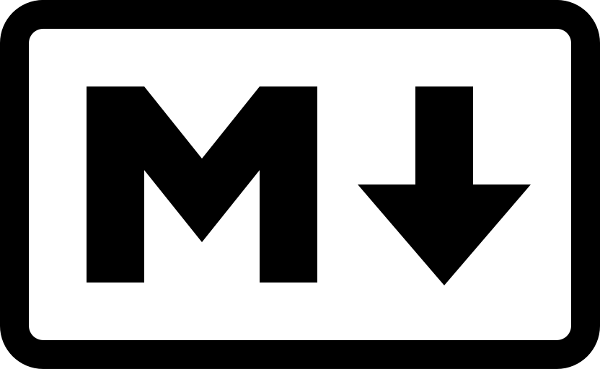
\includegraphics[scale=1]{images/markdown.png}
%     
\includegraphics[scale=0.35]{images/octocat.png}
%     
\includegraphics[scale=0.35]{images/discourse.png}
% \end{frame}

% \begin{frame}[fragile]
%   \frametitle{Пример документа Markdown}
%   \vspace{0.5cm}
%   \screenshotw{11cm}{md-html.png}
% \end{frame}

% \begin{frame}[fragile]
%   \frametitle{AST для Markdown в Haskell}
%   \begin{block}{Документ}
%     \begin{code}
% type Document = [Block]
%     \end{code}
%   \end{block}
%   \begin{block}{Блок}
%     \begin{code}
% data  Block  = Blank
%              | Header (Int,Line)
%              | Paragraph [Line]
%              | UnorderedList [Line]
%              | BlockQuote [Line]
%     \end{code}
%   \end{block}
% \end{frame}

% \begin{frame}[fragile]
%   \frametitle{AST для Markdown в Haskell}
%   \begin{block}{Строка}
%     \begin{code}
% data Line = Empty | NonEmpty [Inline]    
%     \end{code}
%   \end{block}
%   \begin{block}{Элементы строки}
%     \begin{code}
% data  Inline  = Plain String
%               | Bold String
%               | Italic String
%               | Monospace String    
%     \end{code}
%   \end{block}
% \end{frame}

% \begin{frame}[fragile]
%   \frametitle{Конструирование AST}
%     \begin{block}{Парсер для документа}
%       \vspace{-1.4em}
%       \begin{code}
% doc ::  TM.TextualMonoid t => Parser t Document
% doc =   many block
%         where block =  blank <|> header <|> paragraph 
%                        <|> unorderdList <|> blockquote 
%                        <|> blockMath
%       \end{code}
%       \vspace{-1.45em}
%     \end{block}
%     \begin{block}{Пример парсера для заголовка}
%       \vspace{-1.4em}
%       \begin{code}
% header :: TM.TextualMonoid t => Parser t Block 
% header =  do
%           hashes  <- token $ some $ char '#' 
%           text    <- nonEmptyLine
%           return $ Header (length hashes,text)
%       \end{code}
%     \end{block}
% \end{frame}

% \begin{frame}[fragile]
%   \frametitle{Результаты}
%   \begin{enumerate}
%     \item Разработана библиотека монадических парсеров, полиморфных по входным данным. Акцент сделан на подробность сообщений об ошибках. 
%     \item Разработан транслятор подмножества Markdown с \LaTeX-вставками в HTML.
%     \item Начата разработка библиотеки парсеров, основанных на Extensible Effects.
%     \item Исходный код доступен в Git-репозиториях: \\
%         \small{\url{https://github.com/geo2a/markdown_monparsing}} \\
%         \small{\url{https://github.com/geo2a/ext-effects-parsers}}
%   \end{enumerate}
% \end{frame}

\end{document}
